\documentclass[12pt]{article}

\usepackage{amsmath, mathtools}
\usepackage{amsfonts}
\usepackage{amssymb}
\usepackage{babel}
\usepackage{graphicx}
\usepackage{colortbl}
\usepackage{xr}
\usepackage{hyperref}
\usepackage{longtable}
\usepackage{xfrac}
\usepackage{tabularx}
\usepackage{float}
\usepackage{siunitx}
\usepackage{booktabs}
\usepackage{caption}
\usepackage{pdflscape}
\usepackage{afterpage}

\usepackage[round]{natbib}

%\usepackage{refcheck}

\hypersetup{
    bookmarks=true,         % show bookmarks bar?
      colorlinks=true,       % false: boxed links; true: colored links
    linkcolor=red,          % color of internal links (change box color with linkbordercolor)
    citecolor=green,        % color of links to bibliography
    filecolor=magenta,      % color of file links
    urlcolor=cyan           % color of external links
}

%% Comments

\usepackage{color}

\newif\ifcomments\commentstrue

\ifcomments
\newcommand{\authornote}[3]{\textcolor{#1}{[#3 ---#2]}}
\newcommand{\todo}[1]{\textcolor{red}{[TODO: #1]}}
\else
\newcommand{\authornote}[3]{}
\newcommand{\todo}[1]{}
\fi

\newcommand{\wss}[1]{\authornote{blue}{SS}{#1}} 
\newcommand{\wxz}[1]{\authornote{cyan}{XZ}{#1}} 
\newcommand{\plt}[1]{\authornote{magenta}{TPLT}{#1}} %For explanation of the template
\newcommand{\an}[1]{\authornote{cyan}{Author}{#1}}

%% Common Parts

\newcommand{\progname}{ProgName} % PUT YOUR PROGRAM NAME HERE %Every program
                                % should have a name


% For easy change of table widths
\newcommand{\colZwidth}{1.0\textwidth}
\newcommand{\colAwidth}{0.13\textwidth}
\newcommand{\colBwidth}{0.82\textwidth}
\newcommand{\colCwidth}{0.1\textwidth}
\newcommand{\colDwidth}{0.05\textwidth}
\newcommand{\colEwidth}{0.8\textwidth}
\newcommand{\colFwidth}{0.17\textwidth}
\newcommand{\colGwidth}{0.5\textwidth}
\newcommand{\colHwidth}{0.28\textwidth}

% Used so that cross-references have a meaningful prefix
\newcounter{defnum} %Definition Number
\newcommand{\dthedefnum}{GD\thedefnum}
\newcommand{\dref}[1]{GD\ref{#1}}
\newcounter{datadefnum} %Datadefinition Number
\newcommand{\ddthedatadefnum}{DD\thedatadefnum}
\newcommand{\ddref}[1]{DD\ref{#1}}
\newcounter{theorynum} %Theory Number
\newcommand{\tthetheorynum}{T\thetheorynum}
\newcommand{\tref}[1]{T\ref{#1}}
\newcounter{tablenum} %Table Number
\newcommand{\tbthetablenum}{T\thetablenum}
\newcommand{\tbref}[1]{TB\ref{#1}}
\newcounter{assumpnum} %Assumption Number
\newcommand{\atheassumpnum}{P\theassumpnum}
\newcommand{\aref}[1]{A\ref{#1}}
\newcounter{goalnum} %Goal Number
\newcommand{\gthegoalnum}{P\thegoalnum}
\newcommand{\gsref}[1]{GS\ref{#1}}
\newcounter{instnum} %Instance Number
\newcommand{\itheinstnum}{IM\theinstnum}
\newcommand{\iref}[1]{IM\ref{#1}}
\newcounter{reqnum} %Requirement Number
\newcommand{\rthereqnum}{P\thereqnum}
\newcommand{\rref}[1]{R\ref{#1}}
\newcounter{lcnum} %Likely change number
\newcommand{\lthelcnum}{LC\thelcnum}
\newcommand{\lcref}[1]{LC\ref{#1}}

\usepackage{fullpage}

\begin{document}

\title{Software Requirements Specification for Radio Signal Strength Calculator} 
\author{Xingzhi Liu}
\date{\today}
	
\maketitle

~\newpage

\pagenumbering{roman}

\tableofcontents

~\newpage

\section*{Revision History}

\begin{tabularx}{\textwidth}{p{3cm}p{2cm}X}
\toprule {\bf Date} & {\bf Version} & {\bf Notes}\\
\midrule
Oct 5 & 1.0 & First draft of the document\\
Oct 29 & 1.1 & Revision 1 of the document\\
\bottomrule
\end{tabularx}

~\newpage

\section{Reference Material}

This section records information for easy reference.

\subsection{Table of Units}

Throughout this document SI (Syst\`{e}me International d'Unit\'{e}s) is employed
as the unit system.  In addition to the basic units, several derived units are
used as described below.  For each unit, the symbol is given followed by a
description of the unit and the SI name.
~\newline

\renewcommand{\arraystretch}{1.2}
% \begin{table}[ht]
  \noindent \begin{tabular}{l l l} 
    \toprule		
    \textbf{symbol} & \textbf{unit} & \textbf{SI}\\
    \midrule 
    \si{\metre} & length & metre\\
    \si{\metre\per\second} & speed & metre per second\\
    \si{\hertz} & frequency	& hertz\\
    \si{dBm} & power & decibel-milliwatt\\
    \si{\radian} & phase angle & radian\\
    \si{\watt} & power & watt (W = \si{\joule\per\second})\\
    \bottomrule
  \end{tabular}
  % \caption{Table of Units}
% \end{table}


\subsection{Table of Symbols}

The table that follows summarizes the symbols used in this document along with
their units.  The choice of symbols was made to be mostly consistent with the radio
frequency literature and with existing documentation for radio wave propagation
models.

\renewcommand{\arraystretch}{1.2}
%\noindent \begin{tabularx}{1.0\textwidth}{l l X}
\noindent \begin{longtable*}{l l p{12cm}} \toprule
\textbf{symbol} & \textbf{unit} & \textbf{description}\\
\midrule 
$(x,y)$ & \si[per-mode=symbol] {\metre} & Cartesian Position Coordinates in a 2-
dimensional space
\\
$d_\text{a,b}$ & \si[per-mode=symbol] {\metre} & Euclidean Distance between point 
a and point b in a 2-D space
\\
$\Delta d$ & \si[per-mode=symbol] {\metre} & Difference between two travelling 
paths of a radio signal
\\
$\lambda$ & \si[per-mode=symbol] {\metre} & Signal wavelength
\\
$tsm$ & \si[per-mode=symbol] {-} & Transmitter
\\
$Pos_\text{tsm}$ & \si[per-mode=symbol] {\metre} & 2-D position of the transmitter 
\\
$G_{tsm}$ & \si[per-mode=symbol] {\decibel} & Directional gain of the transmitter's 
antenna 
\\
$sp$ & \si[per-mode=symbol] {-} & Sampling point
\\
$Pos_\text{sp}$ & \si[per-mode=symbol] {\metre} & 2-D position of the sampling 
point 
\\
$G_{sp}$ & \si[per-mode=symbol] {\decibel} & Directional gain of the antenna on 
the receiver located at the sampling point
\\
$p$ & \si[per-mode=symbol] {m} & A point
\\
$p'$ & \si[per-mode=symbol] {m} & Mirror point of point $p$
\\
$t$ & \si[per-mode=symbol] {m} & A randomly picked point on the reflection plane
\\
$t'$ & \si[per-mode=symbol] {m} & The point where the line passing the point $p$
and its mirror point $p'$ intersects the reflection plane
\\
$Ind_{r,x}$ & \si[per-mode=symbol] {-} & A boolean indicating whether the reflected signal's path is valid or not
\\
$Ind_{t,x}$ & \si[per-mode=symbol] {-} & A boolean indicating whether the segment of the signal's path intersects wall x or not
\\
$D_t$ & \si[per-mode=symbol] {\decibel} & Directional gain of the transmitter's antenna
\\
$D_r$ & \si[per-mode=symbol] {\decibel} & Directional gain of the receiver's antenna
\\
$n$ & \si[per-mode=symbol] {-} & Unit normal vector of a plane
\\
$i$ & \si[per-mode=symbol] {-} & Imaginary unit
\\
$n_x$ & \si[per-mode=symbol] {-} & Unit normal vector of wall x
\\
$C_x, D_x$ & \si[per-mode=symbol] {\metre} & Starting and ending vertices of wall x in the 2-D space
\\
$x_{C_x},x_{D_x}$ & \si[per-mode=symbol] {\metre} & x-Coordinates of vertices $C_x$ and $D_x$
\\
$y_{C_x},y_{D_x}$ & \si[per-mode=symbol] {\metre} & y-Coordinates of vertices $C_x$ and $D_x$
\\
$E, F$ & \si[per-mode=symbol] {\metre} & Starting and ending vertices of a signal path 
in the 2-D space
\\
$x_{E},x_{F}$ & \si[per-mode=symbol] {\metre} & x-Coordinates of vertices $E$ and $F$
\\
$y_{E},y_{F}$ & \si[per-mode=symbol] {\metre} & y-Coordinates of vertices $E$ and $F$
\\
$M$ & \si[per-mode=symbol] {-} & Coefficient matrix of a line's equation in 2-D space
\\
$m1,m2$ & \si[per-mode=symbol] {-} & Components in in matrix M
\\
$k$ & \si[per-mode=symbol] {\meter} & Coefficient of a line's equation in 2-D space
\\
$\overline{C_x D_x}$ & \si[per-mode=symbol] {\metre} & The line segment representing 
wall x in the 2-D space
\\
$N_w$ & \si[per-mode=symbol] {-} & Total number of walls
\\
$N_r$ & \si[per-mode=symbol] {-} & Total number of first-order reflected signals
\\
$P^{dBm}$ & \si[per-mode=symbol] {dBm} & Power in dBm
\\
$P_{tsm}$ & \si[per-mode=symbol] {\watt} & Power level of the transmitter
\\
$P_{tsm}^{dBm}$ & \si[per-mode=symbol] {dBm} & Power level of the transmitter in dBm
\\
$P_{sp}$ & \si[per-mode=symbol] {\watt} & Received signal strength
\\
$P_{sp}^{dBm}$ & \si[per-mode=symbol] {dBm} & Received signal strength in dBm
\\
$FSPL$ & \si[per-mode=symbol] {-} & Free-space path loss of radio energy
\\
$FSPL_{tsm\rightarrow t'}$ & \si[per-mode=symbol] {-} & Free-space path loss of 
energy of the radio signal travelling from the transmitter to the point $t'$
\\
$R$ & \si[per-mode=symbol] {-} & Wall reflectance
\\
$T$ & \si[per-mode=symbol] {-} & Wall transmittance
\\
$R_x$ & \si[per-mode=symbol] {-} & Reflectance of wall x
\\
$T_x$ & \si[per-mode=symbol] {-} & Transmittance of wall x
\\
$L_{e,\Omega}^i$& \si[per-mode=symbol] {\watt} & Spectral radiance received by 
surface $\Omega$
\\
$L_{e,\Omega}^t$& \si[per-mode=symbol] {\watt} & Spectral radiance passed through 
surface $\Omega$
\\
$L_{e,\Omega}^r$& \si[per-mode=symbol] {\watt} & Spectral radiance reflected by 
surface $\Omega$
\\
$c$ & \si[per-mode=symbol] {\metre/\second} & Speed of light
\\
$f$ & \si[per-mode=symbol] {\hertz} & Signal frequency
\\
$HP$ & \si[per-mode=symbol] {-} & A hyperplane in a Euclidean space
\\
$\phi$ & \si[per-mode=symbol] {\radian} & Phase angle of a wave
\\
$\Delta \phi$ & \si[per-mode=symbol] {\radian} & Phase difference between two waves
\\
$\phi_{sum}$ & \si[per-mode=symbol] {\radian} & Phase angle of the combined wave
\\
$\phi_{FORS}$ & \si[per-mode=symbol] {\radian} & Phase angle of the first-order
reflected signal
\\
$\phi_{sp}$ & \si[per-mode=symbol] {\radian} & Phase angle of received signal
at the sampling point
\\
$A$ & \si[per-mode=symbol] {-} & Amplitude of a sinusoidal wave
\\
$A_{sum}$ & \si[per-mode=symbol] {-} & Amplitude of the combined wave
\\
$A''$ & \si[per-mode=symbol] {\watt} & Complex power of a radio signal
\\
$x$ & \si[per-mode=symbol] {\metre} & The x coordinate in the Cartesian coordinate 
system
\\
$y$ & \si[per-mode=symbol] {\metre} & The y coordinate in the Cartesian coordinate 
system
\\
$LOS$ & \si[per-mode=symbol] {-} & Line-of-sight signal
\\
$FORS$ & \si[per-mode=symbol] {-} & First-order reflected signal
\\
$RS1$ & \si[per-mode=symbol] {-} & Pre-reflection signal
\\
$RS2$ & \si[per-mode=symbol] {-} & Post-reflection signal
\\
$P_{LOS}$ & \si[per-mode=symbol] {\watt} & Power of Line-of-sight signal
\\
$P_{FORS}$ & \si[per-mode=symbol] {\watt} & Power of First-order reflected signal
\\
$P_{RS1}$ & \si[per-mode=symbol] {\watt} & Power of Pre-reflection signal
\\
$P_{RS2}$ & \si[per-mode=symbol] {\watt} & Power of Post-reflection signal
\\
\bottomrule
\end{longtable*}

\subsection{Abbreviations and Acronyms}

\renewcommand{\arraystretch}{1.2}
\begin{tabular}{l l} 
  \toprule		
  \textbf{symbol} & \textbf{description}\\
  \midrule 
  A & Assumption\\
  DD & Data Definition\\
  GD & General Definition\\
  GS & Goal Statement\\
  IM & Instance Model\\
  LC & Likely Change\\
  PS & Physical System Description\\
  R & Requirement\\
  SRS & Software Requirements Specification\\
  RSSC & Radio Signal Strength Calculator for indoor wireless communication systems\\
  T & Theoretical Model\\
  2-D & 2-Dimensional\\
  \bottomrule
\end{tabular}\\

\newpage

\pagenumbering{arabic}

\section{Introduction}

\paragraph{} From the evaluation of Wi-Fi signal coverage to indoor localization, 
radio signal strength is an essential information in various application scenarios 
of indoor wireless communication systems. However, collecting signal strength data 
in the real world is both expensive and time-consuming. We intend to develop a 
tool to simulate the indoor transmission of a radio signal and obtain the signal's strength, hence avoiding expensive on-field surveys.
\paragraph{} The following section provides an overview of the Software Requirements Specification (SRS) for Radio signal Strength Calculator for indoor wireless communication systems (RSSC). This section explains the purpose of this document, 
the scope of the requirements, the characteristics of intended readers, and the 
organization of the document.

\subsection{Purpose of Document}
The essential purpose of this document is to clarify the purpose and requirements 
for RSSC. This document also specifies the assumptions, theoretical models, science definitions and other model derivation information to help the reader understand 
and verify the purpose and scientific basis of RSSC.


\subsection{Scope of Requirements} 

  The scope of requirements includes analysis of the radio signal transmission 
  in a 2 - Dimensional space inside a room. 

\subsection{Characteristics of Intended Reader} \label{sec_IntendedReader}
  Intended readers are supposed to have a technical background in radio frequency 
  engineering. They should be familiar with telecommunication systems; they 
  should understand basic concepts in electromagnetism and optics (covered
  by undergraduate level 1 engineering physics); they should understand undergraduate 
  level 2 engineering mathematics.

\subsection{Organization of Document}
This document follows the standard pattern of presenting goals, assumptions, theories, and definitions. For readers that would like a more bottom up approach, they can start reading 
the instance models in \ref{sec_instance} and trace back to find any additional 
information they require.\\

The goal statement (\ref{gGoalStatement}) is refined to the theoretical models(\ref{sec_theoretical}) and further, to the instance models (\autoref{sec_instance}),
with definitions of data (\ref{sec_datadef}) needed to construct instance models.
The instance models provide the set of algebraic equations that must be solved.
 


\section{General System Description}

This section provides general information about the system.  It identifies the
interfaces between the system and its environment, describes the user
characteristics and lists the system constraints.

\subsection{System Context}

The system context is shown in \autoref{Fig_SystemContext}: RSSC takes inputs from
the user and handle all the calculations within itself, then provides outputs to 
the user. The arrows show the data flow between RSSC and the environment.

\begin{figure}[h!]
\begin{center}
 \includegraphics[width=0.8\textwidth]{Untitled}
\caption{System Context}
\label{Fig_SystemContext} 
\end{center}
\end{figure}

\begin{itemize}
\item User Responsibilities:
\begin{itemize}
\item Provide correct inputs including transmitter settings, wall properties,
and sampling locations to RSSC
\item Ensure the \hyperref[sec_assumpt]{software assumptions} satisfy the 
problem that the user wants to solve
\end{itemize}
\item RSSC Responsibilities:
\begin{itemize}
\item Detect data type mismatch, such as a string of characters instead of a
  floating point number
\item Determine if the input data satisfy the system's \hyperref[sec_DataConstraints]{constraints for input data} or not
\item Calculate signal strength at each sampling point provided by the user
\end{itemize}
\end{itemize}

\subsection{User Characteristics} \label{SecUserCharacteristics}

The end user of RSSC should have an understanding of undergraduate Level 1
physics; should know what is a Cartesian coordinate system, and should be able
to read floor map of a building.

\subsection{System Constraints}
There are no system constraints.

\section{Specific System Description}

This section first presents the problem description, which gives a high-level
view of the problem to be solved; then provides the solution's characteristic
specification, including the assumptions, theories, definitions and
the instance models.

\subsection{Problem Description} \label{Sec_pd}

RSSC is intended to simulate transmission of a radio signal in a room, and 
predict the received signal strength at any location in that room where the 
user wants to measure.

\subsubsection{Terminology and  Definitions}
This subsection provides a list of terms that are used in the subsequent
sections and their meaning, with the purpose of reducing ambiguity and making it
easier to correctly understand the requirements:

\begin{itemize}

\item Radio signal: Also known as radio wave, a type of electromagnetic radiation
with a frequency range from 30Hz to 300GHz. In wireless communication systems, 
radio signals are a medium to transmit information between devices.
\item Transmitter: Source of any radio signals. A transmitter is an electronic 
device that sends a radio signal by injecting a current into its antenna. 
\item Power level of the transmitter: Power of the current fed into the transmitter's antenna.
\item Receiver: An electronic device that receives radio signals from transmitters.
A radio signal generates an electric current in a receiver through the receiver's 
antenna.
\item Received signal strength: Power of the current that the radio signal from a 
given transmitter generates in the given receiver.
\item Antenna: A circuit to transfer radio signals into electric current or vice 
versa.
\item Isotropic Antenna: A type of antenna whose sending efficiency and receiving sensitivity are not affected by its orientation.  
\item Sampling Point: The position where a measurement is taken. In RSSC,
sampling points are where the user wants to locate the simulated receivers and 
find the received signal strengths.
\item Line of sight signal: The radio signal that travels in a straight line 
from the transmitter to the receiver.
\item $k^{th}$-order reflected signal: The radio signal that takes $k$ times of reflection travelling from the transmitter to the receiver.
\end{itemize}

\subsubsection{Physical System Description} \label{sec_phySystDescrip}

The physical system of RSSC, as shown in \autoref{Fig_exampleFloorMap},
includes the following elements:

\begin{itemize}

\item[PS1:] All walls of a room, but not including floor and ceiling.

\item[PS2:] One transmitter.

\item[PS3:] One or more receivers.

\end{itemize}

\begin{figure}[h!]
\begin{center}
 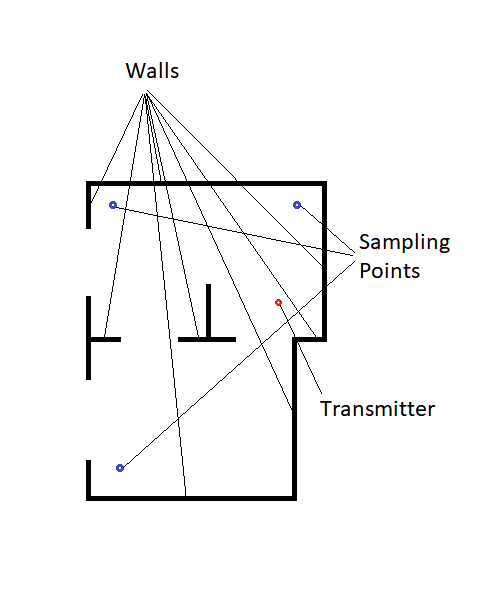
\includegraphics[width=0.6\textwidth]{floorPlan}
\caption{Example Floor Map}
\label{Fig_exampleFloorMap} 
\end{center}
\end{figure}


\subsubsection{Goal Statements} \label{gGoalStatement}

\noindent Given the location and power level of the transmitter, the frequency of the transmitting signal, a list of all walls of a room with their dimensions, locations, transmittance, and reflectance, and a list of sampling points with their locations, the goal statement is:

\begin{itemize}

\item[GS\refstepcounter{goalnum}\thegoalnum \label{goalRSS}:] Calculate
the received signal strength in dBm at each sampling point.

\end{itemize}

\subsection{Solution Characteristics Specification}

The instance models that govern RSSC are presented in
Subsection~\ref{sec_instance}.  The information to understand the meaning of the
instance models and their derivation is also presented, so that the instance
models can be verified.

\subsubsection{Assumptions} \label{sec_assumpt}

This section simplifies the original problem and helps in developing the
theoretical model by filling in the missing information for the physical
system. The numbers given in the square brackets refer to the theoretical model
[T], general definition [GD], data definition [DD], instance model [IM], or
likely change [LC], in which the respective assumption is used.

\begin{itemize}

\item[A\refstepcounter{assumpnum}\theassumpnum \label{2dSpace1}:]
 The space to simulate radio signal transmission is a 2-dimensional space 
 parallel to the room's floor. (Ref.\ By \tref{ED}, \ddref{UNV}, \iref{findN}, 
 \iref{eqnX}, \iref{eqnP}, \iref{RfI}, \iref{TrI})

\item[A\refstepcounter{assumpnum}\theassumpnum \label{2dSpace2}:]
 there are no reflections from the ceiling or the floor. (Ref.\ By \iref{FORS}, 
 \iref{FORP}, \iref{RSS})
 
\item[A\refstepcounter{assumpnum}\theassumpnum \label{mirrorOnly}:]
 Radio signals do not have diffuse reflections. (Ref.\ By \ddref{RA}, 
 \tref{ISM}, \iref{FORS}, \iref{RSS})
 
\item[A\refstepcounter{assumpnum}\theassumpnum \label{isotropy1}:]
 Transmitters have isotropic antennas (received signal strength is independent 
 to the orientation of the transmitter). (Ref.\ By \dref{FSPL})
 
\item[A\refstepcounter{assumpnum}\theassumpnum \label{isotropy2}:]
 Receivers have isotropic antennas (received signal strength is independent 
 to the orientation of the receiver). (Ref.\ By \dref{FSPL})
 
\item[A\refstepcounter{assumpnum}\theassumpnum \label{noThickness}:]
 Walls have no thickness. (Ref.\ By \ddref{TA}, \dref{PDF})
 
\item[A\refstepcounter{assumpnum}\theassumpnum \label{flatWall}:]
 Walls are planar. (Ref.\ By \ddref{RA}, \tref{ISM}, \tref{UNV}, \tref{eqnX},
 , \tref{RfI}, \tref{TrI})
 
\item[A\refstepcounter{assumpnum}\theassumpnum \label{notZero}:]
 Walls have positive lengths. (Ref.\ By \iref{eqnX}, \iref{eqnP}, \iref{findN}, 
 \iref{RfI}, , \tref{TrI})
 
\item[A\refstepcounter{assumpnum}\theassumpnum \label{noMultiReflection}:]
 $2^{nd}$-or-higher-order reflected signals are negligible. (Ref.\ By \iref{RSS})
 
\item[A\refstepcounter{assumpnum}\theassumpnum \label{SingleSource}:]
 Only one transmitter appears in each analysis/simulation case.  (Ref.\ By \dref{WI}, \iref{RSS}))
 
\item[A\refstepcounter{assumpnum}\theassumpnum \label{Sinusoidal}:]
 Waveform for all radio signals are sinusoidal. (Ref.\ By \iref{FORP}, \dref{WI})A

\end{itemize}

\subsubsection{Theoretical Models}\label{sec_theoretical}

This section focuses on the general equations and laws that RSSC is based
on.

~\newline

\noindent
\begin{minipage}{\textwidth}
\renewcommand*{\arraystretch}{1.5}
\begin{tabular}{| p{\colAwidth} | p{\colBwidth}|}
  \hline
  \rowcolor[gray]{0.9}
  Number& T\refstepcounter{theorynum}\thetheorynum \label{ED}\\
  \hline
  Label&\bf Euclidean Distance in 2-D Space\\
  \hline
  Equation&  $d_\text{a,b}$ = $\sqrt{(x_a-x_b)^2+(y_a-y_b)^2}$ for $(x,y)_a$ = 
  $(x_a,y_a)$ and $(x,y)_b$ = $(x_b,y_b)$\\
  \hline
  Description & The above equation gives the Euclidean distance between point
  a and point b as a function of Cartesian position coordinates of point a 
  and point b.
                \\
  \hline
  Source &
           \cite{ED}\\
  % The above web link should be replaced with a proper citation to a publication
  \hline
  Ref.\ By & \dref{PDF}, \dref{FSPL}, \iref{FORP}, \iref{RfI}\\
  \hline
\end{tabular}
\end{minipage}\\

~\newline

\noindent
\begin{minipage}{\textwidth}
\renewcommand*{\arraystretch}{1.5}
\begin{tabular}{| p{\colAwidth} | p{\colBwidth}|}
  \hline
  \rowcolor[gray]{0.9}
  Number& T\refstepcounter{theorynum}\thetheorynum \label{ISM}\\
  \hline
  Label&\bf Image Source Model\\
  \hline
  Equation&  $p'$ = $p-2n(n\cdot(p-t))$ \\ 
  \hline
  Description& The spectral reflection of a plane with unit normal vector $n$
  generates a virtual point $p'$ for a real point $p$. Such $p'$ can be found by 
  the above equation. t is a randomly picked point on the reflection plane. 
  In a 2-D space (according to assumption \aref{2dSpace1}), the reflection plane is a 
  line and $t$ should be on that line.\\
  \hline
  Source & \cite{ISM}\\
  % The above web link should be replaced with a proper citation to a publication
  \hline
  Ref.\ By & \iref{RfI}, \iref{FORS}\\
  \hline
\end{tabular}
\end{minipage}\\

~\newline

\noindent
\begin{minipage}{\textwidth}
\renewcommand*{\arraystretch}{1.5}
\begin{tabular}{| p{\colAwidth} | p{\colBwidth}|}
  \hline
  \rowcolor[gray]{0.9}
  Number& T\refstepcounter{theorynum}\thetheorynum \label{FRIIS}\\
  \hline
  Label&\bf Friis Transmission Formula\\
  \hline
  Equation& $P_{sp}$ = $\frac{P_{tsm} G_{tsm} G_{sp} \lambda^2}{(4 \pi d_{tsm,sp})^2}$ \\
  \hline
  Description& The Friis Transmission Formula is a fundamental equation in radio 
  propagation theory. The formula illustrates the relationship between received 
  signal strength ($P_{sp}$), power level of the transmitter ($P_{tsm}$), directional
  gains of transmitter' and receiver's antennas ($G_{tsm}$ and $G_{sp}$), signal 
  wavelength ($\lambda$), and distance between the transmitter and the receiver 
  ($d_{tsm,sp}$).\\
  \hline
  Source & \cite{FRIIS}\\
  % The above web link should be replaced with a proper citation to a publication
  \hline
  Ref.\ By & \ddref{FSPL}\\
  \hline
\end{tabular}
\end{minipage}\\

\subsubsection{General Definitions}\label{sec_gendef}

This section collects the laws and equations that will be used in building the
instance models.

~\newline

\noindent
\begin{minipage}{\textwidth}
\renewcommand*{\arraystretch}{1.5}
\begin{tabular}{| p{\colAwidth} | p{\colBwidth}|}
  \hline
  \rowcolor[gray]{0.9}
  Number& GD\refstepcounter{defnum}\thedefnum \label{WI}\\
  \hline
  Label&\bf Wave Superposition\\
  \hline
  Units& \si{\watt}\\
  \hline
  Equation&  $A_{sum} e^{i\phi_{sum}}$ = $\sum_{n=1}^{N} A_ne^{i\phi_n}$ for N waves
  from n = 1 to n = N\\
  \hline
  Description & Multiple sinusoidal waves at the  same point will superpose and add 
  together as a combined wave. Here each wave is represented as a phasor with an 
  amplitude A and a phase angle $\phi$. Addition of sinusoidal waves is the same as addition of 
  complex numbers in polar form. \\
  \hline
  Source &
           \cite{WI}\\
  % The above web link should be replaced with a proper citation to a publication
  \hline
  Ref.\ By & \iref{RSS}\\
  \hline
\end{tabular}
\end{minipage}\\

~\newline

\noindent
\begin{minipage}{\textwidth}
\renewcommand*{\arraystretch}{1.5}
\begin{tabular}{| p{\colAwidth} | p{\colBwidth}|}
  \hline
  \rowcolor[gray]{0.9}
  Number& GD\refstepcounter{defnum}\thedefnum \label{PDF}\\
  \hline
  Label&\bf Phase Difference And Path Difference Equation\\
  \hline
  Units& \si{\radian}\\
  \hline
  Equation&  $\Delta \phi$ = $\frac{2\pi \Delta d}{\lambda}$ \\
  \hline
  Description & A wave have different phases when it travels over different distances. 
  The relation between phase difference and distance difference is linear. This equation
  gives the phase difference of two fractions of a signal as a function against the 
  difference between the length of the signal fractions' travelling paths.  \\
  \hline
  Source & \cite{PDF}\\
  % The above web link should be replaced with a proper citation to a publication
  \hline
  Ref.\ By & \iref{FORP}\\
  \hline
\end{tabular}
\end{minipage}\\

\noindent
\begin{minipage}{\textwidth}
\renewcommand*{\arraystretch}{1.5}
\begin{tabular}{| p{\colAwidth} | p{\colBwidth}|}
\hline
\rowcolor[gray]{0.9}
Number& GD\refstepcounter{defnum}\thedefnum \label{FSPL}\\
\hline
Label &\bf Free Space Path Loss Model\\
\hline
SI Units& {-}\\
\hline
Equation&$ FSPL = \frac{P_{tsm}}{P_{sp}} = (\frac{4\pi d_{tsm,sp}}{\lambda})^2 = 
(\frac{4\pi f d_{tsm,sp}} {c})^2$  \\
\hline
Description &
The equation of free space path loss is derived from Friis Transmission Formula (\tref{FRIIS}). According to assumptions \aref{isotropy1} and \aref{isotropy2}, directional gains of antennas are always equal to 1. The free space path loss 
($FSPL$) gives the ratio of the power level of the transmitter to the received 
signal strength in an environment without any obstacles. A larger value of $FSPL$
indicates a higher power loss in signal propagation.
\\
\hline
  Source & \cite{FSPL} \\
  \hline
  Ref.\ By & \iref{LOSS}, \iref{FORS}\\
  \hline
\end{tabular}
\end{minipage}\\

\subsubsection*{Detailed derivation of simplified rate of change of temperature}

\subsubsection{Data Definitions}\label{sec_datadef}

This section collects and defines all the data needed to build the instance
models. The dimension of each quantity is also given.
~\newline

\noindent
\begin{minipage}{\textwidth}
\renewcommand*{\arraystretch}{1.5}
\begin{tabular}{| p{\colAwidth} | p{\colBwidth}|}
  \hline
  \rowcolor[gray]{0.9}
  Number& DD\refstepcounter{datadefnum}\thedatadefnum \label{RA}\\
  \hline
  Label&\bf Reflectance\\
  \hline
  Symbol& $R$\\
  \hline
  Units & {-}\\
  \hline
  Equation&  $R$ = $\frac{L_{e,\Omega}^r}{L_{e,\Omega}^i}$ \\
  \hline
  Description& Reflectance of a surface is the ratio of the reflected radiance's 
  power of a surface ($L_{e,\Omega}^r$) to the power of the radiance went into 
  that surface ($L_{e,\Omega}^i$). \\
  \hline
  Source & \cite{RA}\\
  % The above web link should be replaced with a proper citation to a publication
  \hline
  Ref.\ By & \iref{FORS}\\
  \hline
\end{tabular}
\end{minipage}\\

~\newline

\noindent
\begin{minipage}{\textwidth}
\renewcommand*{\arraystretch}{1.5}
\begin{tabular}{| p{\colAwidth} | p{\colBwidth}|}
  \hline
  \rowcolor[gray]{0.9}
  Number& DD\refstepcounter{datadefnum}\thedatadefnum \label{TA}\\
  \hline
  Label&\bf Transmittance\\
  \hline
  Symbol& $T$\\
  \hline
  Units & {-}\\
  \hline
  Equation&  $T$ = $\frac{L_{e,\Omega}^t}{L_{e,\Omega}^i}$ \\
  \hline
  Description& Reflectance of a wall is the ratio of the power of the radiance that
  transmitted through the wall ($L_{e,\Omega}^t$) to the power of the radiance went 
  into that wall ($L_{e,\Omega}^i$). \\
  \hline
  Source & \cite{TA}\\
  % The above web link should be replaced with a proper citation to a publication
  \hline
  Ref.\ By & \iref{LOSS},\iref{FORS}\\
  \hline
\end{tabular}
\end{minipage}\\

~\newline

\noindent
\begin{minipage}{\textwidth}
\renewcommand*{\arraystretch}{1.5}
\begin{tabular}{| p{\colAwidth} | p{\colBwidth}|}
  \hline
  \rowcolor[gray]{0.9}
  Number& DD\refstepcounter{datadefnum}\thedatadefnum \label{UNV}\\
  \hline
  Label&\bf Unit Normal Vector\\
  \hline
  Symbol& $n$\\
  \hline
  Units & {-}\\
  \hline
  Equation&  $n$ = $\frac{\nabla F}{|| F ||}$ \\
  \hline
  Description& The unit normal vector of a surface is a vector perpendicular to that  
  surface and have a magnitude of 1.\\
  \hline
  Source & \cite{UNV}\\
  % The above web link should be replaced with a proper citation to a publication
  \hline
  Ref.\ By & \tref{ISM}, \iref{findN}\\
  \hline
\end{tabular}
\end{minipage}\\

~\newline

\noindent
\begin{minipage}{\textwidth}
\renewcommand*{\arraystretch}{1.5}
\begin{tabular}{| p{\colAwidth} | p{\colBwidth}|}
  \hline
  \rowcolor[gray]{0.9}
  Number& DD\refstepcounter{datadefnum}\thedatadefnum \label{dbmToWatt}\\
  \hline
  Label&\bf Decibel-Milliwatt\\
  \hline
  Symbol& $P^{dBm}$\\
  \hline
  Units & {dBm}\\
  \hline
  Equation&  $P^{dBm}$ = $30 + 10\log_{10} \frac{P}{1\si{\watt}}$ \\
  & $P = 1\si{\watt} \cdot 10^{\frac{P^{dBm}-30}{10}}$\\
  \hline
  Description& dBm is a unit to represent the magnitude of power. In RSSC, the 
  transmitter power level in the user input and received signal strength in the
  output are in dBm.\\
  \hline
  Source & \cite{DBM}\\
  % The above web link should be replaced with a proper citation to a publication
  \hline
  Ref.\ By & \iref{LOSS}, \iref{FORS}\\
  \hline
\end{tabular}
\end{minipage}\\

\subsubsection{Instance Models} \label{sec_instance}    

This section transforms the problem defined in Section~\ref{Sec_pd} into 
one which is expressed in mathematical terms. It uses concrete symbols defined 
in Section~\ref{sec_datadef} to replace the abstract symbols in the models 
identified in Sections~\ref{sec_theoretical} and~\ref{sec_gendef}.

~\newline

%Instance Model 1

\noindent
\begin{minipage}{\textwidth}
\renewcommand*{\arraystretch}{1.5}
\begin{tabular}{| p{\colAwidth} | p{\colBwidth}|}
  \hline
  \rowcolor[gray]{0.9}
  Number& IM\refstepcounter{instnum}\theinstnum \label{eqnX}\\
  \hline
  Label& \bf Equation Of Wall x\\
  \hline
  Input& $C_x$ and $D_x$ of wall x from the user \\
  &($C_x$ and $D_x$ should not be at the same location) (\aref{notZero})\\
  \hline
  Output&$M = \begin{pmatrix}
  m1 & m2 \\
\end{pmatrix}$ and $k$ for the equation representing the wall's line: $M \begin{pmatrix}
  x & y \\
\end{pmatrix}^T = k$\\
  \hline
  Description& $C_x = (x_{C_x},y_{C_x})$ is the position of wall x's starting vertex. (\si{\meter}).\\
  &$D_x = (x_{D_x},y_{D_x})$ is the position of wall x's ending vertex. (\si{\meter}).\\
  &$M = \begin{pmatrix}
  m1 & m2 \\
\end{pmatrix}$ is the coefficient matrix of the equation of wall x, in which
\\
  &$$ m1 =
  \begin{cases}
  -\frac{y_{D_x}-y_{C_x}}{x_{D_x}-x_{C_x}} & $if $ x_{D_x}-x_{C_x}\neq{0}\\
  1 & $else$\\
  \end{cases}
  $$ and $$ m2 =
  \begin{cases}
  1 & $if $ x_{D_x}-x_{C_x}\neq{0}\\
  0 & $else$\\
  \end{cases}
  $$\\
  &$k$ is a coefficient in the line's equation(\si{\meter}), and can be calculated 
  as following:\\  
  &$k = m1\cdot x_{C_x} + m2\cdot y_{C_x} = m1\cdot x_{D_x} + m2\cdot y_{D_x}$\\
  \hline
  Sources& \cite{eqnX} \\
  \hline
  Ref.\ By & \iref{FORS}, \iref{FORP}, \iref{LOSS}\\
  \hline
\end{tabular}
\end{minipage}\\
%~\newline

\subsubsection*{Derivation of the line's equation}
$M \begin{pmatrix}
  x & y \\
\end{pmatrix}^T = k$\\
$\begin{pmatrix}
  m1 & m2 \\
\end{pmatrix}
\begin{pmatrix}
  x & y \\
\end{pmatrix}^T = k$\\
\\
$m1 \cdot x + m2 \cdot y = k$\\
\\
if $ x_{D_x}-x_{C_x}\neq{0}$: \\
\\
\indent
$m2\cdot y = -m1\cdot x + k$\\
\\
\indent
$y = -\frac{m1}{m2}\cdot x + \frac{k}{m2}$\\
\\
In which $-\frac{m1}{m2}$ is the slope of the function of y against x, and $\frac{k}{m2}$ 
is the y-intercept of the function y against x.\\
\\
For the equation of a line:\\
\\
\indent
$y = \frac{\Delta Y}{\Delta X} x + y(0)$\\ 
\\
Where $\frac{\Delta Y}{\Delta X}$ is the slope of the line and $y(0)$ is the value of y
when x = 0. In the equation above, $\Delta X$ is the change of x-value and $\Delta Y$ 
is the corresponding change in y-value. In RSSC, we can take the difference between the starting and the ending vertices' x-Coordinates as $\Delta X$ and take the difference between the starting and the ending vertices' y-Coordinates as $\Delta Y$, then we 
have:\\
\\
\indent
$\frac{\Delta Y}{\Delta X} = -\frac{m1}{m2} = \frac{y_{D_x}-y_{C_x}}{x_{D_x}-x_{C_x}}$\\
\\
For lines that are not vertical (In RSSC, $ x_{D_x}-x_{C_x} \neq 0$), we can set $m2$ 
to $1$, then:\\
\\
\indent
$y = -m1\cdot x + k$\\
\\
\indent
$m1 = -\frac{y_{D_x}-y_{C_x}}{x_{D_x}-x_{C_x}}$\\
\\
if $x_{D_x}-x_{C_x} = 0$, we will not be able to find $m1$ by $m1 = -\frac{y_{D_x}-y_{C_x}}{x_{D_x}-x_{C_x}}$ since we cannot take 0 as the denominator. In this case, we preliminarily set $m1 = 1$. Then:\\
\\
\indent
$k = m1\cdot x_{C_x} + m2\cdot y_{C_x} = m1\cdot x_{D_x} + m2\cdot y_{D_x}$\\
\\
\indent
$k = 1\cdot x_{C_x} + m2\cdot y_{C_x} = 1\cdot x_{D_x} + m2\cdot y_{D_x}$\\
\\
Since $x_{D_x}-x_{C_x} = 0$, $x_{C_x} = x_{D_x}$, so\\
\\
\indent
$m2\cdot y_{C_x} =  m2\cdot y_{D_x}$\\
\\
Also because $y_{C_x} \neq y_{D_x}$ (\aref{notZero}), the only solution for $m2$ is\\
\\
\indent
$m2 = 0$\\

~\newline

\noindent
\begin{minipage}{\textwidth}
\renewcommand*{\arraystretch}{1.5}
\begin{tabular}{| p{\colAwidth} | p{\colBwidth}|}
  \hline
  \rowcolor[gray]{0.9}
  Number& IM\refstepcounter{instnum}\theinstnum \label{eqnP}\\
  \hline
  Label& \bf Equation Of Signal Path\\
  \hline
  Input& $E$ and $F$ of wall x from the user or \iref{RfI} \\
  \hline
  Output&$M = \begin{pmatrix}
  m1 & m2 \\
\end{pmatrix}$ and $k$ for the equation of the line representing the signal path: $M \begin{pmatrix}
  x & y \\
\end{pmatrix}^T = k$\\
  \hline
  Description& $E = (x_{E},y_{E})$ is the position of the signal path's starting vertex. (\si{\meter}).\\
  &$F = (x_{F},y_{F})$ is the position of the signal path's ending vertex. (\si{\meter}).\\
  &Strategy to find $m1$, $m2$, and $k$ here is the same as in (\iref{eqnX}).\\
  \hline
  Sources& \cite{eqnX} \\
  \hline
  Ref.\ By & \iref{FORS}, \iref{FORP}, \iref{LOSS}\\
  \hline
\end{tabular}
\end{minipage}\\
%~\newline
  
%Instance Model 2
~\newline
\noindent
\begin{minipage}{\textwidth}
\renewcommand*{\arraystretch}{1.5}
\begin{tabular}{| p{\colAwidth} | p{\colBwidth}|}
  \hline
  \rowcolor[gray]{0.9}
  Number& IM\refstepcounter{instnum}\theinstnum \label{findN}\\
  \hline
  Label& \bf Unit Normal Vector For Wall x\\
  \hline
  Input& $C_x$ and $D_x$ of wall x from the user \\
  &($C_x$ and $D_x$ should not be at the same location) (\aref{notZero})\\
  \hline
  Output&$n$ of wall x\\
  \hline
  Description& $C_x = (x_{C_x},y_{C_x})$ is the position of wall x's starting vertex. (\si{\meter}).\\
  &$D_x = (x_{D_x},y_{D_x})$ is the position of wall x's ending vertex. (\si{\meter}).\\
  &$n$ is the unit normal vector of wall x and can be calculated as below:\\
  &$n = \begin{bmatrix}
  (x_{D_x}-x_{C_x}) & (y_{D_x}-y_{C_x})\\
  \end{bmatrix}$
  $\begin{bmatrix}
  0 & -1\\
  1 & 0
  \end{bmatrix} \cdot \frac{1}{\sqrt{(y_{D_x}-y_{C_x})^2+(x_{D_x}-x_{C_x})^2}}
  $\\
  \hline
  Sources& \cite{UNV} \\
  \hline
  Ref.\ By & \iref{RfI}, \iref{TrI}, \iref{FORS}, \iref{FORP}\\
  \hline
\end{tabular}
\end{minipage}\\

\subsubsection*{Derivation of the equation of $n$}
Let $A = (x_{D_x}-x_{C_x})$, let $B = (y_{D_x}-y_{C_x})$;\\
The vector representing wall x's line segment is then:\\
\indent
$\begin{pmatrix}
A & B \\
\end{pmatrix}$\\
By the definition given in (\ddref{UNV}), n is perpendicular to the wall, so the dot product of n and $(A$  $B)$ should be equal to 0.\\
proof:\\
\\
\indent
$n = \begin{bmatrix}
  (x_{D_x}-x_{C_x}) & (y_{D_x}-y_{C_x})\\
  \end{bmatrix}$
  $\begin{bmatrix}
  0 & -1\\
  1 & 0
  \end{bmatrix} \cdot \frac{1}{\sqrt{(y_{D_x}-y_{C_x})^2+(x_{D_x}-x_{C_x})^2}}
  $\\
  \\
  \indent
  $n = \begin{bmatrix}
  A & B\\
  \end{bmatrix}$
  $\begin{bmatrix}
  0 & -1\\
  1 & 0
  \end{bmatrix} \cdot \frac{1}{\sqrt{(y_{D_x}-y_{C_x})^2+(x_{D_x}-x_{C_x})^2}}
  $\\
  \\
  Since $C_x$ and $D_x$ are not at the same location (\aref{notZero}), we can 
  conclude that\\
  \\
  \indent
  $\sqrt{(y_{D_x}-y_{C_x})^2+(x_{D_x}-x_{C_x})^2} > 0$\\
  \\
  Also,\\
  \\
  \indent
  $\begin{bmatrix}
  A & B\\
  \end{bmatrix}$
  $\begin{bmatrix}
  0 & -1\\
  1 & 0
  \end{bmatrix}$ = 
  $\begin{bmatrix}
  B & -A\\
  \end{bmatrix}$, and\\
  \\
  \indent
  $||\begin{bmatrix}
  B & -A\\
  \end{bmatrix}|| = \sqrt{B^2+(-A)^2} = \sqrt{(y_{D_x}-y_{C_x})^2+(x_{D_x}-x_{C_x})^2}$\\
  \\
  So $|| n || =  \frac{\sqrt{(y_{D_x}-y_{C_x})^2+(x_{D_x}-x_{C_x})^2}}{\sqrt{(y_{D_x}-y_{C_x})^2+(x_{D_x}-x_{C_x})^2}} = 1$.\\
  \\
  Let q = $\frac{1}{\sqrt{(y_{D_x}-y_{C_x})^2+(x_{D_x}-x_{C_x})^2}}$,
  \\
  \\
  \indent
  $n \cdot \begin{bmatrix}
  A & B\\
  \end{bmatrix} = \begin{bmatrix}
  B & -A\\
  \end{bmatrix} \cdot \begin{bmatrix}
  A & B\\
  \end{bmatrix} \cdot q$
  \\
  \indent
  $n \cdot \begin{bmatrix}
  A & B\\
  \end{bmatrix} = [AB + (-AB)] \cdot q$
  \\
  \indent
  $n \cdot \begin{bmatrix}
  A & B\\
  \end{bmatrix} = 0 \cdot q$
  \\
  \indent
  $n \cdot \begin{bmatrix}
  A & B\\
  \end{bmatrix} = 0$
  \\
  
~\newline
\noindent
\begin{minipage}{\textwidth}
\renewcommand*{\arraystretch}{1.5}
\begin{tabular}{| p{\colAwidth} | p{\colBwidth}|}
  \hline
  \rowcolor[gray]{0.9}
  Number& IM\refstepcounter{instnum}\theinstnum \label{RfI}\\
  \hline
  Label& \bf Reflection Intersection\\
  \hline
  Input&$C_x$, $D_x$ of wall x from the user (\si{\metre})\\
  &$Pos_{tsm}$, $Pos_{sp}$ from the user (\si{\metre})\\
  &$n$ from \iref{findN}\\ 
  &$M_x$,$k_x$ from \iref{eqnX}\\
  &$M_p$,$k_p$ from \iref{eqnP}\\
  &($C_x$ and $D_x$ should not be at the same location) (\aref{notZero})\\
  
  \hline
  Output&$t'$\\
  &$Ind_{r,x}$\\
  &$d_{rsm',sp}$ \\
  \hline
  Description&$C_x = (x_{C_x},y_{C_x})$ is the position of wall x's starting vertex (\si{\meter}).\\
  &$D_x = (x_{D_x},y_{D_x})$ is the position of wall x's ending vertex (\si{\meter}).\\
  &$Pos_{tsm}$ is the position of the transmitter (\si{\meter}).\\
  &$Pos_{sp}$ is the position of the sampling point (\si{\meter}).\\
  &$n$ is the unit normal vector of wall x given by \iref{findN}.\\ 
  &$t'$ is the point on wall x's plane where the signal to reflect intersects 	
  that plane (t' may not be on wall x. wall x has limited dimensions, and t' may
  fall outside of wall x, but still on wall x's plane) (\si{\metre}).\\
  &$Ind_{r,x}$ is a boolean which indicates whether wall x intersects t' or not.\\ 
  &Use $C_x$, $Pos_{tsm}$, and $n$ to find $Pos_{tsm}$'s mirror point $Pos'_{tsm}$	  
  (refer to \tref{ISM}).\\
  &Solve the linear system $\begin{pmatrix}
  M_x \\
  M_p
  \end{pmatrix}
  \begin{pmatrix}
  x \\
  y
  \end{pmatrix}$ = $
  \begin{pmatrix}
  k_x \\
  k_p
  \end{pmatrix}$ for $\begin{pmatrix}
  x \\
  y
  \end{pmatrix}$. $x$ and $y$ here are coordinates of $t'$.\\
  &$M_x$ and $k_x$ in the linear system above are coefficients of the line equation for wall x.\\
  &$M_p$ and $k_p$ in the linear system above are coefficients of the line equation for the signal path from $Pos'_{tsm}$ to $Pos_{sp}$.\\
  &$Ind_{r,x} = 
  \begin{cases}
  1 & $ if $ min(x_{C_x},x_{D_x}) < x < max(x_{C_x},x_{D_x})$ and $\\
  & min(y_{C_x},y_{D_x}) < y < max(y_{C_x},y_{D_x})\\
  0 & else\\
  \end{cases}$\\
  &$d_{rsm',sp}$ is the Euclidean distance between the mirror of the transmitter at 
  $Pos'_{tsm}$ and the sampling point at $Pos_{sp}$ (\si{\metre}).\\
  \hline
  Sources& \cite{RfI} \\
  \hline
  Ref.\ By & \iref{FORS}, \iref{FORP}\\
  \hline
\end{tabular}
\end{minipage}\\

~\newline
\noindent
\begin{minipage}{\textwidth}
\renewcommand*{\arraystretch}{1.5}
\begin{tabular}{| p{\colAwidth} | p{\colBwidth}|}
  \hline
  \rowcolor[gray]{0.9}
  Number& IM\refstepcounter{instnum}\theinstnum \label{TrI}\\
  \hline
  Label& \bf Transmission Intersection\\
  \hline
  Input& $C_x$, $D_x$, and $R_x$ of wall x from the user\\
  &$E$, $F$ from the user or (\iref{RfI})\\
  &$M_x$,$k_x$ from (\iref{eqnX})\\
  &$M_p$,$k_p$ from (\iref{eqnP})\\
  &($C_x$ and $D_x$ should not be at the same location) (\aref{notZero})\\
  
  \hline
  Output&$Ind_{t,x}$ that indicates whether wall x intersects the signal's path or 
  not.\\
  \hline
  Description& $C_x = (x_{C_x},y_{C_x})$ is the position of wall x's starting vertex. 
  (\si{\meter}).\\
  &$D_x = (x_{D_x},y_{D_x})$ is the position of wall x's ending vertex. (\si{\meter}).\\
  &$n$ is the unit normal vector of wall x given by \iref{findN}.\\  
  &Solve the linear system $\begin{pmatrix}
  M_x \\
  M_p
  \end{pmatrix}
  \begin{pmatrix}
  x \\
  y
  \end{pmatrix}$ = $
  \begin{pmatrix}
  k_x \\
  k_p
  \end{pmatrix}$ for $\begin{pmatrix}
  x \\
  y
  \end{pmatrix}$.\\  
  &$M_x$ and $k_x$ in the linear system above are coefficients of the line equation for wall x.\\
  &$M_p$ and $k_p$ in the linear system above are coefficients of the line equation for the signal path from $E$ to $F$.\\
  &$Ind_{t,x} = 
  \begin{cases}
  1 & $ if $ min(x_{C_x},x_{D_x}) < x < max(x_{C_x},x_{D_x})$ and $\\
  & min(y_{C_x},y_{D_x}) < y < max(y_{C_x},y_{D_x})\\
  0 & else\\
  \end{cases}$\\
  \hline
  Sources& \cite{RfI} \\
  \hline
  Ref.\ By & \iref{LOSS}, \iref{FORS}, \iref{FORP}\\
  \hline
\end{tabular}
\end{minipage}\\

~\newline
\noindent
\begin{minipage}{\textwidth}
\renewcommand*{\arraystretch}{1.5}
\begin{tabular}{| p{\colAwidth} | p{\colBwidth}|}
  \hline
  \rowcolor[gray]{0.9}
  Number& IM\refstepcounter{instnum}\theinstnum \label{LOSS}\\
  \hline
  Label& \bf Line Of Sight Signal Strength\\
  \hline
  Input
  &$f$ of the radio signal from user \\
  &$d_{tsm,sp}$ from (\tref{ED})\\
  &A list of [$T_x$] for all walls ($x=1,2,\cdots ,N_w$) from the user\\
  &A list of [$Ind_{t,x}$] for all walls ($x=1,2,\cdots ,N_w$) from (\iref{TrI})\\
  &$P_{tsm}^{dBm}$ from the user\\
  
  \hline
  Output
  &$P_{LOS}$\\
  \hline
  Description
  & $f$ is the frequency of the radio signal (\si{\hertz}).\\
  & $T_x$ is the transmittance of wall x.\\
  &[$T_x$] is an ($N_w \times 1$) list of $T_x$ for $x=1,2,\cdots ,N_w$.\\
  & $Ind_{t,x}$ is a boolean. $Ind_{t,x}$ = 1 if wall x occludes the line of sight 
  signal's path, otherwise $Ind_{t,x}$ = 0.\\
  &[$Ind_{t,x}$] is an ($N_w \times 1$) list of $Ind_{t,x}$ for $x=1,2,\cdots ,N_w$.\\
  &$N_w$ is the total number of walls.\\
  &$P_{tsm}^{dBm}$ is the power level of the transmitter (dBm).\\
  &$P_{LOS}$ is the power of line of sight signal in \si{\watt}.\\
  &First transfer power in dBm to power in \si{\watt} (\ddref{dbmToWatt}).\\
  &Use $f$ and $d_{tsm,sp}$ to find $FSPL$ (\dref{FSPL}).\\
  &The power of line of sight signal can be derived as:\\
  &$P_{LOS} = \frac{P_{tsm}}{FSPL}\cdot \prod_{x=1}^{N_w}T_x^{(Ind_{t,x})}$\\
  &\\
  \hline
  Sources& \cite{RfI}, \cite{DBM} \\
  \hline
  Ref.\ By & \iref{RSS}, \iref{FORS}\\
  \hline
\end{tabular}
\end{minipage}\\

\subsubsection*{Derivation of the equation of $P_{LOS}$}

The definition of transmittance $T$ is the ratio of the power of radiance passing 
through the obstacle to the power of radiance as if there was no obstacle(\ddref{TA}).
If there are multiple obstacles, The power of radiance that passes through all the
obstacles will be the initial power of the radiance times the percentage of power 
passing through the first obstacle, then times the percentage of power 
passing through the second obstacle and so on. So we have $\prod_{x=1}^{N_w}T_x$ in 
the calculation of line of sight signal strength.\\
\\
The reason to take $Ind_{t,x}$ as the power of $T_x$ is that not all of the walls 
appear in a signal's path. For walls not blocking the signal, we should not let them
attenuate the signal in the simulation. When wall x blocks the signal, $Ind_{t,x}$ 
= 1 (\iref{TrI}), in this case $T_x^{(Ind_{t,x})} = T_x$. When wall x does
not block the signal, $Ind_{t,x}$ = 0 and $T_x^{(Ind_{t,x})} = 1$, meaning that no
power loss happens due to wall x.\\
\\
Radio signals attenuate not only due to material transmittance, but also due to travelling in space. According to (\dref{FSPL}), $\frac{1}{FSPL}$ is the ratio of the signal's power after travelling a distance $d$ in free space. This attenuation should also be included
in our calculation.\\
\\
Considering the above, the line of sight signal strength is hence:\\ 
\indent
$P_{LOS} = \frac{P_{tsm}}{FSPL}\cdot \prod_{x=1}^{N_w}T_x^{(Ind_{t,x})}$.
 
~\newline
\noindent
\begin{minipage}{\textwidth}
\renewcommand*{\arraystretch}{1.5}
\begin{tabular}{| p{\colAwidth} | p{\colBwidth}|}
  \hline
  \rowcolor[gray]{0.9}
  Number& IM\refstepcounter{instnum}\theinstnum \label{FORS}\\
  \hline
  Label& \bf First-Order Reflected Signal Strength\\
  \hline
  Input
  &$f$ of the radio signal from user \\
  &A list of [$T_x$] for all walls ($x=1,2,\cdots ,N_w$) from the user\\
  &A list of [$Ind_{t,x}$] for all walls ($x=1,2,\cdots ,N_w$) from (\iref{TrI})\\
  &$R_x$ for wall x from the user\\
  &$Ind_{r,x}$ for wall x from (\iref{RfI})\\
  &$t'$ for wall x from (\iref{RfI})\\
  &$P_{tsm}^{dBm}$ from the user\\
  &$Pos_{tsm}$ from the user\\
  &$Pos_{sp}$ from the user\\
  
  \hline
  Output
  &$P_{FROS_x}$\\
  \hline
  Description
  &$f$ is the frequency of the radio signal (\si{\hertz}).\\
  &$Pos_{tsm}$ is the position of the transmitter (\si{\meter}).\\
  &$Pos_{sp}$ is the position of the sampling point (\si{\meter}).\\
  & $T_x$ is the transmittance of wall x.\\
  &[$T_x$] is an ($N_w \times 1$) list of $T_x$ for $x=1,2,\cdots ,N_w$.\\
  & $Ind_{t,x}$ is a boolean. $Ind_{t,x}$ = 1 if wall x occludes the line of sight 
  signal's path, otherwise $Ind_{t,x}$ = 0.\\
  &[$Ind_{t,x}$] is an ($N_w \times 1$) list of $Ind_{t,x}$ for $x=1,2,\cdots ,N_w$.\\
  &$N_w$ is the total number of walls.\\
  &$R_x$ is the reflectance of wall x (\ddref{RA}).\\
  &$Ind_{r,x}$ is a boolean indicating whether wall x intersects t' or not. 
  (\iref{RfI})\\
  &$t'$ is the point on wall x's plane where the signal to reflect intersects that
  plane (\iref{RfI}). (\si{\meter})\\
  &$P_{tsm}^{dBm}$ is the power level of the transmitter (dBm).\\
  \hline
\end{tabular}
\end{minipage}\\

~\newline
\noindent
\begin{minipage}{\textwidth}
\renewcommand*{\arraystretch}{1.5}
\begin{tabular}{| p{\colAwidth} | p{\colBwidth}|}
  \hline
  Label& \bf First-Order Reflected Signal Strength\\
  \hline
  Description Continued  
  &$P_{FROS_x}$ is the power of first-order reflected signal that travels from $Pos_{tsm}$,
  has a specular reflection at wall x , then reaches $Pos_{sp}$ (\si{\watt}).\\
  &Transfer power in dBm to power in \si{\watt} (\ddref{dbmToWatt}).\\
  &Use $f$ and $d_{tsm,sp}$ to find $FSPL$ (\dref{FSPL}).\\
  &The first-order reflected signal can be divided into 2 sections: Pre-Reflection signal 
  ($RS1$) and Post-Reflection signal ($RS2$).\\ 
  &For Pre-Reflection signal, calculation of its power $P_{RS1}$ is the same as 
  calculation of $P_{LOS}$, but $Pos_{sp}$ is replaced with the position of $t'$ here.\\
  &Pre-Reflection signal at $t'$ is the source of Post-Reflection signal. With 
  reflectance, transmittance, and path loss, the resulting power of Post-Reflection 
  signal is then:\\
  &$P_{RS2}$ = $\frac{P_{tsm}}{FSPL_{tsm\rightarrow t'}}\prod_{i=1}^{N_w} T_i^{(Ind_{t,i})}\times R_x \times Ind_{r,i}\times\frac{1}{FSPL_{t'\rightarrow sp}}\prod_{j=1}^{N_w} T_j^{(Ind_{t,j})}$\\
  &and $P_{FROS_x}$ = $P_{RS2}$\\
  \hline
  Sources& \cite{RfI} \\
  \hline
  Ref.\ By & \iref{RSS}\\
  \hline
\end{tabular}
\end{minipage}\\

~\newline
\noindent
\begin{minipage}{\textwidth}
\renewcommand*{\arraystretch}{1.5}
\begin{tabular}{| p{\colAwidth} | p{\colBwidth}|}
  \hline
  \rowcolor[gray]{0.9}
  Number& IM\refstepcounter{instnum}\theinstnum \label{FORP}\\
  \hline
  Label& \bf First-Order Reflection Signal Phase Angle\\
  \hline
  Input
  &$f$ of the radio signal from user \\
  &$d_{tsm,sp}$ from (\tref{ED})\\
  &$d_{tsm,t'}$ from (\tref{ED})\\
  &$d_{t',sp}$ from (\tref{ED})\\
  
  \hline
  Output
  &$\phi_{FORS_x}$\\
  \hline
  Description
  & $f$ is the frequency of the radio signal (\si{\hertz}).\\
  &$d_{tsm,sp}$ is the Euclidean distance between the transmitter and the receiver (\si{\meter}).\\
  &$d_{tsm,t'}$ is the Euclidean distance between the transmitter and the point $t'$ (\si{\meter}).\\
  &$d_{t',sp}$ is the Euclidean distance between the the point $t'$ and the receiver (\si{\meter}).\\
  &$t'$ is the point on wall x's plane where the signal to reflect intersects that
  plane (\iref{RfI}). (\si{\meter})\\
  &$\phi_{FORS_x}$ is the phase angle of the first-order reflected signal against 
  wall x, when taking the line of sight signal as a reference with 0\si{\radian} 
  phase angle.\\
  &According to \dref{PDF}, $\phi_{FORS_x}$ can be found by the following equation:\\
  &$\phi_{FORS_x} = \frac{2\pi f (d_{tsm,t'}+d_{t',sp}-d_{tsm,sp})}{c}$\\
  \hline
  Sources& \cite{RfI}, \cite{DBM} \\
  \hline
  Ref.\ By & \iref{RSS}\\
  \hline
\end{tabular}
\end{minipage}\\

\subsubsection*{Derivation of the equation of $\phi_{FORS_x}$}

\indent
$\Delta \phi = \frac{2\pi \Delta d}{\lambda}$\\
\\
\indent
$\phi_{FORS_x}-\phi_{LOS} = \frac{2\pi \Delta d}{\lambda}$\\
\\
\indent
$\phi_{FORS_x}-\phi_{LOS} = \frac{2\pi f \Delta d}{c}$\\
\\
\indent
$\phi_{FORS_x}-\phi_{LOS} = \frac{2\pi f (d_{tsm,t'}+d_{t',sp}-d_{tsm,sp})}{c}$\\
\\
\indent
$\phi_{FORS_x} = \frac{2\pi f (d_{tsm,t'}+d_{t',sp}-d_{tsm,sp})}{c}$ as $\phi_{LOS} = 0$\\

~\newline
\noindent
\begin{minipage}{\textwidth}
\renewcommand*{\arraystretch}{1.5}
\begin{tabular}{| p{\colAwidth} | p{\colBwidth}|}
  \hline
  \rowcolor[gray]{0.9}
  Number& IM\refstepcounter{instnum}\theinstnum \label{RSS}\\
  \hline
  Label& \bf Received Signal Strength\\
  \hline
  Input
  &$P_{LOS}$ from (\iref{LOSS})\\
  &[$P_{FROS_x}$] for $x = 1,2,3,\cdots,N_w$ from (\iref{FORS})\\
  &[$\phi_{FORS_x}$] for $x = 1,2,3,\cdots,N_w$ from (\iref{FORP})\\
  
  \hline
  Output
  &$P_{sp}^{dBm}$\\
  \hline
  Description
  &$P_{LOS}$ is the line of sight signal strength (\si{\watt}).\\
  &$P_{FROS_x}$ is the first-order reflected signal strength (\si{\watt}).\\
  &$\phi_{FORS_x}$ is the phase angle of the first-order reflected signal against 
  wall x, when taking the line of sight signal as a reference with 0\si{\radian} 
  phase angle.\\
  &According to \tref{WI},\\
  &$P_{sp}e^{i\phi_{sp}}=P_{LOS}e^0 + \sum_{x=1}^{N_w} P_{FROS_x}e^{i\phi_{FORS_x}}$\\
  &$P_{sp}^{dBm} =  30+10\log_{10}(\frac{P_{sp}}{1W})$\\
  \hline
  Sources& \cite{WI}, \cite{DBM} \\
  \hline
  Ref.\ By & \gsref{goalRSS}\\
  \hline
\end{tabular}
\end{minipage}\\

\subsubsection{Input Data Constraints} \label{sec_DataConstraints}    

Table~\ref{TblInputVar} shows the data constraints on the input output
variables.  The column for physical constraints gives the physical limitations
on the range of values that can be taken by the variable.  The column for
software constraints restricts the range of inputs to reasonable values.  The
software constraints will be helpful in the design stage for picking suitable
algorithms.  The constraints are conservative, to give the user of the model the
flexibility to experiment with unusual situations.  The column of typical values
is intended to provide a feel for a common scenario.  The uncertainty column
provides an estimate of the confidence with which the physical quantities can be
measured.  This information would be part of the input if one were performing an
uncertainty quantification exercise.

The specification parameters in Table~\ref{TblInputVar} are listed in
Table~\ref{TblSpecParams}.

\begin{table}[!h]
  \caption{Input Variables} \label{TblInputVar}
  \renewcommand{\arraystretch}{1.2}
\noindent \begin{longtable*}{l l l l c} 
  \toprule
  \textbf{Var} & \textbf{Physical Constraints} & \textbf{Software Constraints} &
                             \textbf{Typical Value} & \textbf{Uncertainty}\\
  \midrule 
  $T_x$ & $0 < T_x < 1$ & N/A & 0.1 & 10\%\\
  $R_x$ & $0 < R_x < 1$ & N/A & 0.6 & 10\%\\
  $P_{tsm}^{dBm}$ & N/A & $P_{min}^{dBm} \leq P_{tsm}^{dBm} \leq P_{max}^{dBm}$ & 0\si{dBm} & 15\%\\
  $f$ & N/A & $f_{min} \leq f \leq {f_max}$ & $2.4\times 10^{9}$\si{\hertz} & 10\%\\
  $x_{C_x}$ &  N/A  & $ x_{min} \leq x_{C_x} \leq x_{max}$ & 0\si{\meter} & 10\%\\
  $y_{C_x}$ &  N/A  & $ y_{min} \leq y_{C_x} \leq y_{max}$ & 0\si{\meter} & 10\%\\
  $x_{D_x}$ &  N/A  & $ x_{min} \leq x_{D_x} \leq x_{max}$ & 0\si{\meter} & 10\%\\
  $y_{D_x}$ &  N/A  & $ y_{min} \leq y_{D_x} \leq y_{max}$ & 0\si{\meter} & 10\%\\
  $N_w$ &  N/A  & $ 0 \leq P_{tsm}^{dBm} \leq \times 10^{11}$ & 0\si{\meter} & 10\%\\
  \\
  \bottomrule
\end{longtable*}
\end{table}

\begin{table}[!h]
\caption{Specification Parameter Values} \label{TblSpecParams}
\renewcommand{\arraystretch}{1.2}
\noindent \begin{longtable*}{l l} 
  \toprule
  \textbf{Var} & \textbf{Value} \\
  \midrule 
  $P_{max}^{dBm}$ & 15 \si{dBm}\\
  $P_{min}^{dBm}$ & -30 \si{dBm}\\
  $f_{min}$ & 30 \si{\hertz}\\
  $f_{max}$ & $3\times 10^{11}$  \si{\hertz}\\
  $x_{min}$ & -20 \si{\meter}\\
  $x_{max}$ & 20 \si{\meter}\\
  $y_{min}$ & -20 \si{\meter}\\
  $y_{max}$ & 20 \si{\meter}\\
  \bottomrule
\end{longtable*}
\end{table}

\subsubsection{Properties of a Correct Solution} \label{sec_CorrectSolution}

\noindent
A correct solution must exhibit the law of conservation of energy. This means that
$P_{sp}^{dBm}$ should always be lower than $P_{tsm}^{dBm}$.

\begin{table}[!h]
\caption{Output Variables} \label{TblOutputVar}
\renewcommand{\arraystretch}{1.2}
\noindent \begin{longtable*}{l l} 
  \toprule
  \textbf{Var} & \textbf{Physical Constraints} \\
  \midrule 
  $P_{sp}^{dBm}$ & $-120 < P_{sp}^{dBm} < 0$ 
  \\
  $Pos_{sp}$ & N/A 
  \\
  \bottomrule
\end{longtable*}
\end{table}

\section{Requirements}

This section provides the functional requirements, the business tasks that the
software is expected to complete, and the nonfunctional requirements, the
qualities that the software is expected to exhibit.

\subsection{Functional Requirements}

\noindent \begin{itemize}

\item[R\refstepcounter{reqnum}\thereqnum \label{R_Inputs}:] RSSC shall input the
data shown in Table \ref{ReqInputVar}, and store the data.

\item[R\refstepcounter{reqnum}\thereqnum \label{R_VerifyInputs}:] Verify that 
the number of starting points, number of ending points, number of directional 
transmittances and directional Reflectances of walls are consistent; verify
that the input Cartesian position coordinates, transmitter power level and signal
frequency are within appropriate range.

\item[R\refstepcounter{reqnum}\thereqnum \label{R_Calculate}:] Calculate and output
the value of $P_{sp}^{dBm}$.

\item[R\refstepcounter{reqnum}\thereqnum \label{R_VerifyOutput}:] Verify 
the value of $P_{sp}^{dBm}$ in the final result. The $P_{sp}^{dBm}$ should never be 
greater than $P_{tsm}^{dBm}$.

\item[R\refstepcounter{reqnum}\thereqnum \label{R_Output}:] Generate a file storing
$P_{sp}^{dBm}$ at every sampling point the user provide.

\end{itemize}

\begin{table}[!h]
\caption{Required Input Variables} \label{ReqInputVar}
\renewcommand{\arraystretch}{1.2}
\noindent \begin{longtable*}{l l c} 
  \toprule
  \textbf{Symbol} & \textbf{Description} & \textbf{Units}\\
  \midrule 
  $Pos_{tsm}$ & Cartesian position coordinates of the transmitter & m\\
  $[Pos_{sp}]$ & (multiple entities) Cartesian position coordinates of sampling points & m\\
  $[C]$ & (multiple entities) Cartesian position coordinates of the starting point of walls & m\\
  $[D]$ & (multiple entities) Cartesian position coordinates of the ending point of walls & m\\
  $[T]$ & (multiple entities) Directional transmittances of walls & -\\
  $[R]$ & (multiple entities) Directional Reflectances of walls & -\\
  $P_{tsm}^{dBm}$ & Power level of the transmitter & dBm\\
  $f$ & frequency of the signal & Hz\\
  \bottomrule
\end{longtable*}
\end{table}

\newpage
\subsection{Nonfunctional Requirements}


\paragraph{Correct:} The outputs of RSSC satisfies the description in \autoref{sec_CorrectSolution}.

\paragraph{Verifiable:} Easy to test and verify.

\paragraph{Portable:} Able to run in different environments.

\paragraph{Maintainable:} Proper documents should be included in this project.

\paragraph{Understandable:} Program of RSSC should be organized, well commented, and easy
to understand.

\section{Likely Changes}    

\noindent \begin{itemize}

\item[LC\refstepcounter{lcnum}\thelcnum\label{HOR}:] The assumption that
2nd-order or higher order reflections are negligible (\aref{noMultiReflection}) 
is too weak. High order reflections of radio signals can have complicated behaviors. 
For example we cannot simulate the effect of a corner reflector with only direct 
and 1st-order reflected signals.

\item[LC\refstepcounter{lcnum}\thelcnum\label{IST}:]  Oriented antennas 
are commonly used on transmitters to enhance the signal strength toward some 
designated directions. To simulate this scenario, we may change the assumption
(\aref{isotropy1}) and introduce directional gains to transmitters.


\item[LC\refstepcounter{lcnum}\thelcnum\label{FCR}:]  Another likely 
change is the assumption that floor and ceiling do not reflect radio signals 
(\aref{2dSpace2}). This assumption was made to simplify the analysis, but floor
and ceiling are strong reflectors. Besides, floor and ceiling reflections
are regular and easy to integrate into the 2-D system.
\end{itemize}

\section{Unlikely Changes}    

\noindent \begin{itemize}

\item[UC1:]  The assumption 
that walls have positive lengths (\aref{notZero}) is unlikely to change because 
a wall with zero or negative length is meaningless both for analysis and in the 
real world.

\end{itemize}

\section{Traceability Matrices and Graphs}

The purpose of the traceability matrices is to provide easy references on what
has to be additionally modified if a certain component is changed.  Every time a
component is changed, the items in the column of that component that are marked
with an ``X'' may have to be modified as well.  Table~\ref{Table:trace} shows the
dependencies of theoretical models, general definitions, data definitions, and
instance models with each other. Table~\ref{Table:R_trace} shows the
dependencies of instance models and requirements on each
other. Table~\ref{Table:A_trace} shows the dependencies of theoretical models,
general definitions, data definitions, instance models, and likely changes on
the assumptions.

\afterpage{
\begin{table}[h!]
\centering
\begin{tabular}{|c|c|c|c|c|c|c|c|c|c|c|c|c|c|c|c|c|c|c|c|}
\hline
	& \aref{2dSpace1}& \aref{2dSpace2}& \aref{mirrorOnly}& \aref{isotropy1}& \aref{isotropy2}& \aref{noThickness}& \aref{flatWall}& \aref{notZero}& \aref{noMultiReflection}& \aref{SingleSource}& \aref{Sinusoidal} \\
\hline
\tref{ED}      	    &X& & & & & & & & & & \\ \hline
\tref{ISM}        	& & &X& & & &X& & & & \\ \hline
\tref{FRIIS}        & & & & & & & & & & & \\ \hline
\dref{WI} 			& & & & & & & & & & &X\\ \hline
\dref{PDF}          & & & & & &X& & & & & \\ \hline
\dref{FSPL}         & & & &X&X& & & & & & \\ \hline
\ddref{RA}		    & & &X& & & &X& & & & \\ \hline
\ddref{TA}     		& & & & & &X& & & & & \\ \hline
\ddref{UNV}       	&X& & & & & &X& & & & \\ \hline
\ddref{dbmToWatt}   & & & & & & & & & & & \\ \hline
\iref{eqnX}         &X& & & & & &X&X& & & \\ \hline
\iref{eqnP}         &X& & & & & & &X& & & \\ \hline
\iref{findN}       	&X& & & & & & & & & & \\ \hline
\iref{RfI}       	&X& & & & & &X&X& & & \\ \hline
\iref{TrI}     		&X& & & & & &X&X& & & \\ \hline
\iref{LOSS}    		& & & & & &X& & & & & \\ \hline
\iref{FORS}  		& &X& & & & & & & & & \\ \hline
\iref{FORP}  		& &X& & & & & & & & &X\\ \hline
\iref{RSS} 			& &X&X& & & & & &X&X& \\ \hline
\lcref{HOR} 		& & & & & & & & &X& & \\ \hline
\lcref{IST} 		& & & &X& & & & & & & \\ \hline
\lcref{FCR}    		& &X& & & & & & & & & \\
\hline
\end{tabular}
\caption{Traceability Matrix Showing the Connections Between Assumptions and Other Items}
\label{Table:A_trace}
\end{table}
}

\afterpage{
\begin{landscape}
\begin{table}[h!]
\centering
\begin{tabular}{|c|c|c|c|c|c|c|c|c|c|c|c|c|c|c|c|c|c|c|c|c|c|c|c|c|c|c|c|}
\hline        
& \tref{ED}& \tref{ISM}& \tref{FRIIS}& \dref{WI}& \dref{PDF}& \dref{FSPL}& \ddref{RA}& \ddref{TA}& \ddref{UNV}& \ddref{dbmToWatt}& \iref{eqnX}& \iref{eqnP}& \iref{findN}& 
\iref{RfI}& \iref{TrI}& \iref{LOSS}& \iref{FORS}& \iref{FORP}& \iref{RSS}\\
\hline
\tref{ED}     		& & & & & & & & & & & & & & & & & & & \\ \hline
\tref{ISM}     		& & & & & & & & &X& & & & & & & & & & \\ \hline
\tref{FRIIS}     	& & & & & & & & & & & & & & & & & & & \\ \hline
\dref{WI}        	& & & & & & & & & & & & & & & & & & & \\ \hline
\dref{PDF}      	&X& & & & & & & & & & & & & & & & & & \\ \hline
\dref{FSPL} 		&X& &X& & & & & & & & & & & & & & & & \\ \hline
\ddref{RA}  		& & & & & & & & & & & & & & & & & & & \\ \hline
\ddref{TA}    		& & & & & & & & & & & & & & & & & & & \\ \hline
\ddref{UNV}     	& & & & & & & & & & & & & & & & & & & \\ \hline
\ddref{dbmToWatt}   & & & & & & & & & & & & & & & & & & & \\ \hline
\iref{eqnX}      	& & & & & & & & & & & & & & & & & & & \\ \hline
\iref{eqnP}    		& & & & & & & & & & & & & & & & & & & \\ \hline
\iref{findN}    	& & & & & & & & &X& & & & & & & & & & \\ \hline
\iref{RfI}    		&X&X& & & & & & & & & & &X& & & & & & \\ \hline
\iref{TrI}    		& & & & & & & & & & & & &X& & & & & & \\ \hline
\iref{LOSS}    		&X& & & & &X& &X& &X&X&X& & &X& & & & \\ \hline
\iref{FORS}    		&X&X& & & &X&X&X& &X&X&X&X&X&X&X& & & \\ \hline
\iref{FORP}    		&X& & & &X& & & & & &X&X&X&X&X& & & & \\ \hline
\iref{RSS}    		&X& & &X& & & & & & & & & & & &X&X&X& \\
\hline
\end{tabular}
\caption{Traceability Matrix Showing the Connections Between Items of Different Sections}
\label{Table:trace}
\end{table}
\end{landscape}
}

\begin{table}[h!]
\centering
\begin{tabular}{|c|c|c|c|c|c|c|c|c|c|c|c|c|c|c|}
\hline
	& \iref{eqnX}& \iref{eqnP}& \iref{findN}& \iref{RfI}& \iref{TrI}& \iref{LOSS}& \iref{FORS}& \iref{FORP}& \iref{RSS}& \rref{R_Inputs}\\
\hline
\iref{eqnX}            	& & & & & & & & & &X\\ \hline
\iref{eqnP}            	& & & & & & & & & &X\\ \hline
\iref{findN}          	& & & & & & & & & &X\\ \hline
\iref{RfI}          	& & &X& & & & & & &X\\ \hline
\iref{TrI}     			& & &X& & & & & & &X\\ \hline
\iref{LOSS}    			&X&X& & &X& & & & &X\\ \hline
\iref{FORS}   			&X&X&X&X&X&X& & & &X\\ \hline
\iref{FORP}  			&X&X&X&X&X& & & & &X\\ \hline
\iref{RSS}     			& & & & & &X&X&X& &X\\ \hline 
\rref{R_Inputs}       	& & & & & & & & & &\\ \hline
\rref{R_VerifyInputs}   & & & & & & & & & &\\ \hline
\rref{R_Calculate}     	&X& & & & & & & &X&\\ \hline
\rref{R_VerifyOutput}  	& & & & & & & & & &\\ \hline
\rref{R_Output} 		& & & & & & & & &X&\\
\hline
\end{tabular}
\caption{Traceability Matrix Showing the Connections Between Requirements and Instance Models}
\label{Table:R_trace}
\end{table}


% \begin{figure}[h!]
% 	\begin{center}
% 		%\rotatebox{-90}
% 		{
% 			\includegraphics[width=\textwidth]{ATrace.png}
% 		}
% 		\caption{\label{Fig_ATrace} Traceability Matrix Showing the Connections Between Items of Different Sections}
% 	\end{center}
% \end{figure}


% \begin{figure}[h!]
% 	\begin{center}
% 		%\rotatebox{-90}
% 		{
% 			\includegraphics[width=0.7\textwidth]{RTrace.png}
% 		}
% 		\caption{\label{Fig_RTrace} Traceability Matrix Showing the Connections Between Requirements, Instance Models, and Data Constraints}
% 	\end{center}
% \end{figure}

\section{Values of Auxiliary Constants}

This section contains the standard values that are used for calculations in RSSC
.
\begin{table}[!h]
\renewcommand{\arraystretch}{1.2}
\noindent \begin{longtable*}{l l c c} 
  \toprule
  \textbf{Symbol} & \textbf{Description} & \textbf{Value} & \textbf{Units}\\
  \midrule 
  $c$ & speed of light & $3\times 10^8$ & \si{\metre\per\s}\\
  \bottomrule
\end{longtable*}
\label{Constant}
\end{table}



\newpage
\bibliographystyle {plainnat}
\bibliography {References}

\end{document}